\section{Galileitransformatie}
%%%%%%%%%%%%
\subsection{Twee inertiaalsystemen}
Twee inertiaalstelsels $S$ en $S'$ zijn verbonden door de 
Galileitransformatie :
\begin{eqnarray*}
x' & = & x + 3t \\ 
y' & = & y \\
z' & = & z \\
t' & = & t 
\end{eqnarray*}
\begin{itemize}
\item [a.] In welke richting beweegt $S$ t.o.v. $S'$?
\item [b.] Schrijf de transformatie-formules op voor de 
snelheidscomponenten
$v_{x}$, $v_{y}$, $v_{z}$.
\end{itemize}
In $S$ duwt een kracht $F$ een voorwerp met massa $m$ 
met een versnelling 
$a = 2 $m/s$^{2}$ voort: van snelheid $v = 4$m/s op 
$t = 0$ en $x = 0$, tot snelheid
$v = 10$m/s op $t = 3$s en $x = 21 $m.
\begin{itemize}
\item [c.]
Welke waarden hebben $a, F, x$ en $v $ in $S'$?
\item [d.]
Blijft de formule $v$ = $v(0)$ + $at$ in $S'$ van kracht?
\end{itemize}
Zowel in $S$ als $S'$ kun je de arbeid $W = F\Delta$x en de groei van de 
kinetische energie $\Delta E_{k}$ = $\Delta (\frac{1}{2}mv^{2})$ uitrekenen.
\begin{itemize}
\item [e.]
Is de arbeid die verricht wordt hetzelfde, gezien vanuit $S$ en $S'$?
\item [f.]
Dezelfde vraag voor $\Delta E_{k}$.
\item [g.]
Geldt zowel in $S$ als in $S'$ dat $F\Delta x$ gelijk is aan 
$\Delta (\frac{1}{2}mv^{2})$?
\item [h.]
Omschrijf nu wat het relativiteitsprincipe inhoudt voor 
Galileitransformaties.
\end{itemize}


%%%%%%%%%%%%
\subsection{Tennissen}
 \begin{figure} [h]
 \begin{center}
 \mbox{\epsfxsize=10cm\epsffile{oefeningen.pictures/tennis.eps}}
 \caption{Tennissen}
 \label{f:tennis}
 \end{center}
 \end{figure}
Een satelliet die zich om een bewegende planeet slingert, krijgt
daarvan een extra snelheid mee, ongeveer zoals een tennisbal dat van een
bewegende tennisracket krijgt. $v_{b}$, $v_{e}$ en $v_{0}$ zijn de
begin-, eind- , planeet/tennisracket-snelheid in het co\"ordinatenstelsel
$S$ van de toeschouwer. $S'$ is het co\"ordinatenstelsel dat met de
planeet/tennisracket meebeweegt.
\begin{itemize}
\item [a.]
Wat zijn de begin- en eindsnelheid van de bal in het 
co\"{o}rdinatenstelsel $S'$?
\end{itemize}
Bij de elastische botsing van de bal met het racket is in $S'$
is de snelheid van de bal na de botsing even groot 
als de snelheid voor de botsing.
\begin{itemize}
\item [b.]
Hoe groot is de eindsnelheid van de bal in $S$ in termen 
van $v_{b}$ en $v_{0}$?
\item [c.]
Hoe verandert de kinetische energie $E_{k} = \frac{1}{2}mv^{2}$ van de bal 
in $S$?
\item[d.] 
En in $S'$?
\end{itemize}
Terwijl  de {\it waarden} van grootheden in $S$ en $S'$ kunnen verschillen, 
moeten de formules tussen de  grootheden  wel {\it invariant} zijn. 
\begin{itemize}
\item [e.]
Laat zien dat de formule $\Delta E_{k} =F\Delta x$ zowel in $S$ als in $S'$ 
geldt (het racket werkt met $F = m_{bal}\frac{\Delta v}{\Delta t}$ over een 
afstand $\Delta x = v_{0} \Delta {t}$).
\end{itemize}
%
%\begin{figure} [h]
%\begin{center}
%\mbox{\epsfxsize=3cm\epsffile{oefeningen.pictures/planet.eps}}
%\caption{}
%\label{f:planeet}
%\end{center}
%\end{figure}

%%%%%%%%%%
\subsection{Een paraboolbaan}

% \begin{figure} [h]
% \begin{center}
% \mbox{\epsfxsize=5cm\epsffile{oefeningen.pictures/parabool.eps}}
% \caption{Paraboolbaan}
% \label{f:parabool}
% \end{center}
% \end{figure}

\begin{figure}[ht]
\centering
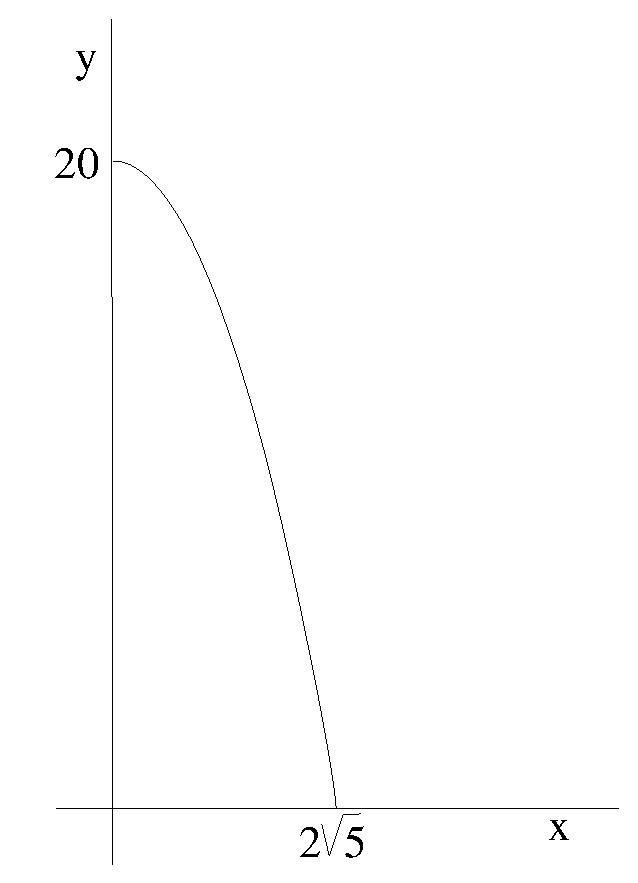
\includegraphics[width=.5\textwidth]{oefeningen.pictures/parabool}
\caption{Paraboolbaan}
\label{f:parabool}
\end{figure}


Gegeven een paraboolbaan (zie figuur \ref{f:parabool}) t.o.v.
co\"{o}rdinatenstelsel $S$:
\begin{displaymath}
y = -x^{2} + 20
\end{displaymath}
Dit is de baan die beschreven wordt door een puntmassa die met een
horizontale beginsnelheid van een 20 meter hoge toren gegooid wordt.
De versnelling van de zwaartekracht is $g = 10$ m/s$^{2}$.
Geef de Galileitransformatie naar stelsel $S'$ zodat de puntmassa t.o.v. dit
stelsel langs een rechte, verticale lijn beweegt.

%%%%%%%%%%%%
\subsection{Versnellende auto}
Als  je  vanuit  een  inertiaalsysteem  een Galileitransformatie uitvoert, 
kom je in een ander inertiaalsysteem.
\begin{itemize}
\item [a.]
Hoe weet je zeker dat je in een inertiaalsysteem bent?
\end{itemize}
Het  interieur van een auto (stelsel $S'$), die versneld door een straat 
(stelsel $S$) rijdt, is g\'{e}\'{e}n  
inertiaalsysteem  en  de transformatie van $S'$ naar $S$ is g\'{e}\'{e}n
Galileitransformatie:    
\begin{eqnarray}
\label{v:auto}
x = x' \pm \frac{1}{2} at^{2}  \\
y = y'  \\
z = z'
\end{eqnarray}

\begin{itemize}
\item [b.]
Moet je in formule \ref{v:auto} het plus- of het minteken nemen?
\item [c.]
Een bal die je binnen in de auto op $t = 0$ loslaat, heeft dan $v = 0$ en 
$v' = 0$.\\
In welk stelsel, $S$ of $S'$ geldt tijdens de val van de bal 
$v_{x} = 0$? 
\item [d.]
Leidt nu uit de transformatieformules  af  hoe de snelheid in $S'$
zich ontwikkelt.
\item [e.]
In  $S'$ is er een versnelling $a_{x}$, en voel je dus
een `kracht' $F_{x }= ma_{x}$.\\
Hoe groot is de kracht en in welke richting werkt de kracht?
\end{itemize}

%%%%%%%%%%%%%
\subsection {Michelson-Morley voor geluid}
V\'{o}\'{o}r  de komst van de speciale relativiteitstheorie veronderstelde 
men dat de lichtsnelheid een vaste  waarde  had in \'{e}\'{e}n 
bepaald inertiaalsysteem (de `ether') en dat de lichtsnelheid in 
andere systemen  via  een  Galileitransformatie kon worden afgeleid. 
Deze veronderstelling bleek niet houdbaar  (zie  o.a.  het  
Michelson-Morley experiment), maar hij geldt {\it wel} voor geluid. 
Vandaar deze opgave, als contrast met de gang van zaken voor licht.

Geluid  heeft  een  vaste  snelheid  t.o.v.  zijn  medium  
(de  lucht,  stelsel $S$),  nl. 
$c_{g} = 1/\sqrt{\rho\kappa}$
waar $\rho$ de dichtheid en $\kappa$ de `compressibiliteit' van de lucht zijn.

% \begin{figure} [h]
% \begin{center}
% \mbox{\epsfxsize=10cm\epsffile{oefeningen.pictures/wind.eps}}
% \end{center}
% \caption{Michelson en Morley voor geluid}
% \label{f:oef1-6}
% \end{figure}

\begin{figure}[ht]
\centering
%\mbox{\epsfxsize=10cm\epsffile{oefeningen.pictures/wind.eps}}
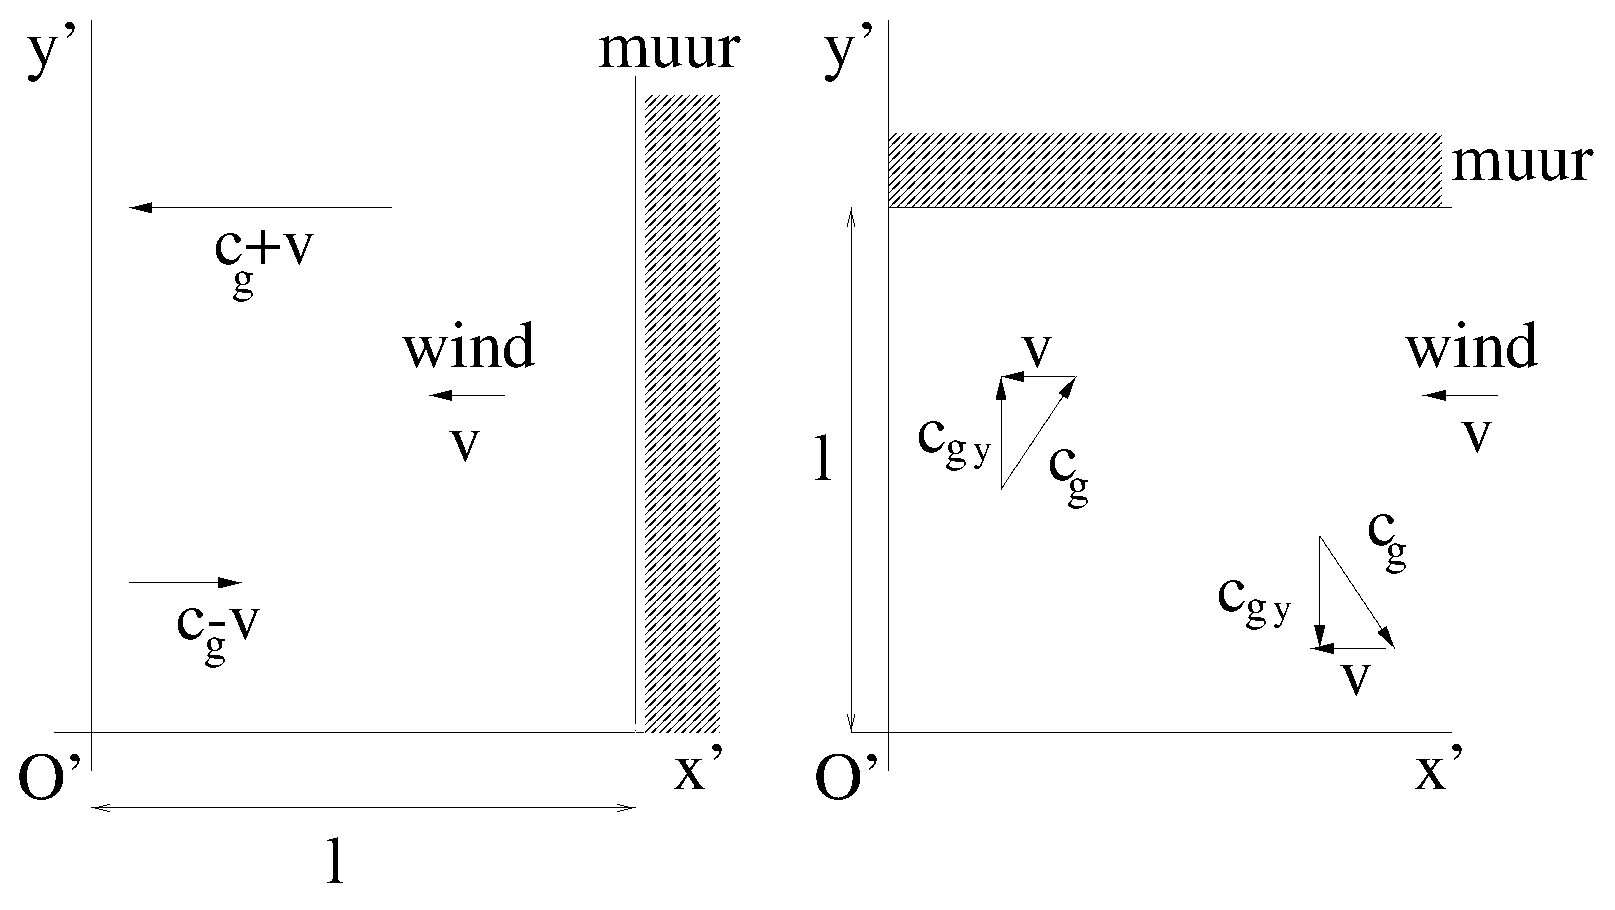
\includegraphics[width=1.0\textwidth]{oefeningen.pictures/wind}
\caption{Michelson en Morley voor geluid}
\label{f:oef1-6}
\end{figure}


Als  in je eigen stelsel ($S'$) de wind je tegemoet blaast met snelheid 
$v$ (of als je met snelheid $v$  naar  voren  beweegt),  is  de  
geluidssnelheid  in  $S'$  volgens de Galileitransformatie gelijk aan 
$c_{g}-v$.\\
We kunnen deze beweging t.o.v. het medium aantonen door de reistijden van het
geluid te meten langs gelijke trajecten in onderling loodrechte
richtingen (de $x'$- en $y'$-as van $S'$).


\begin{itemize}
\item [a.]
  Bereken na hoeveel tijd je de echo uit de $x$-richting en 
  uit de $y$-richting hoort als het windstil is. Is er verschil? 
\end{itemize}
Nu  waait  er  wel  wind,  van  rechts, zoals aangegeven in figuur
\ref{f:oef1-6},
Het geluid moet dan in $S$ schuin naar rechts lopen, om in $S'$ langs 
de $y'$-as heen er weer te gaan (zie figuur \ref{f:oef1-6} rechts).
\begin{itemize}
\item [b.]
Hoeveel tijd kost het nu voor je de echo uit de $x$-richting hoort?
\item [c.]
  En uit de $y$-richting?
\item [d.]
Hoe zou je dus, als je de wind niet zou kunnen voelen of zien, toch kunnen 
constateren dat hij waait? (Neem bijv. $l = 340$m; $v = 20$ m/s en $c_{g} = 340$ m/s)
\end{itemize}

